\begin{figure}[!b]
    \centering
    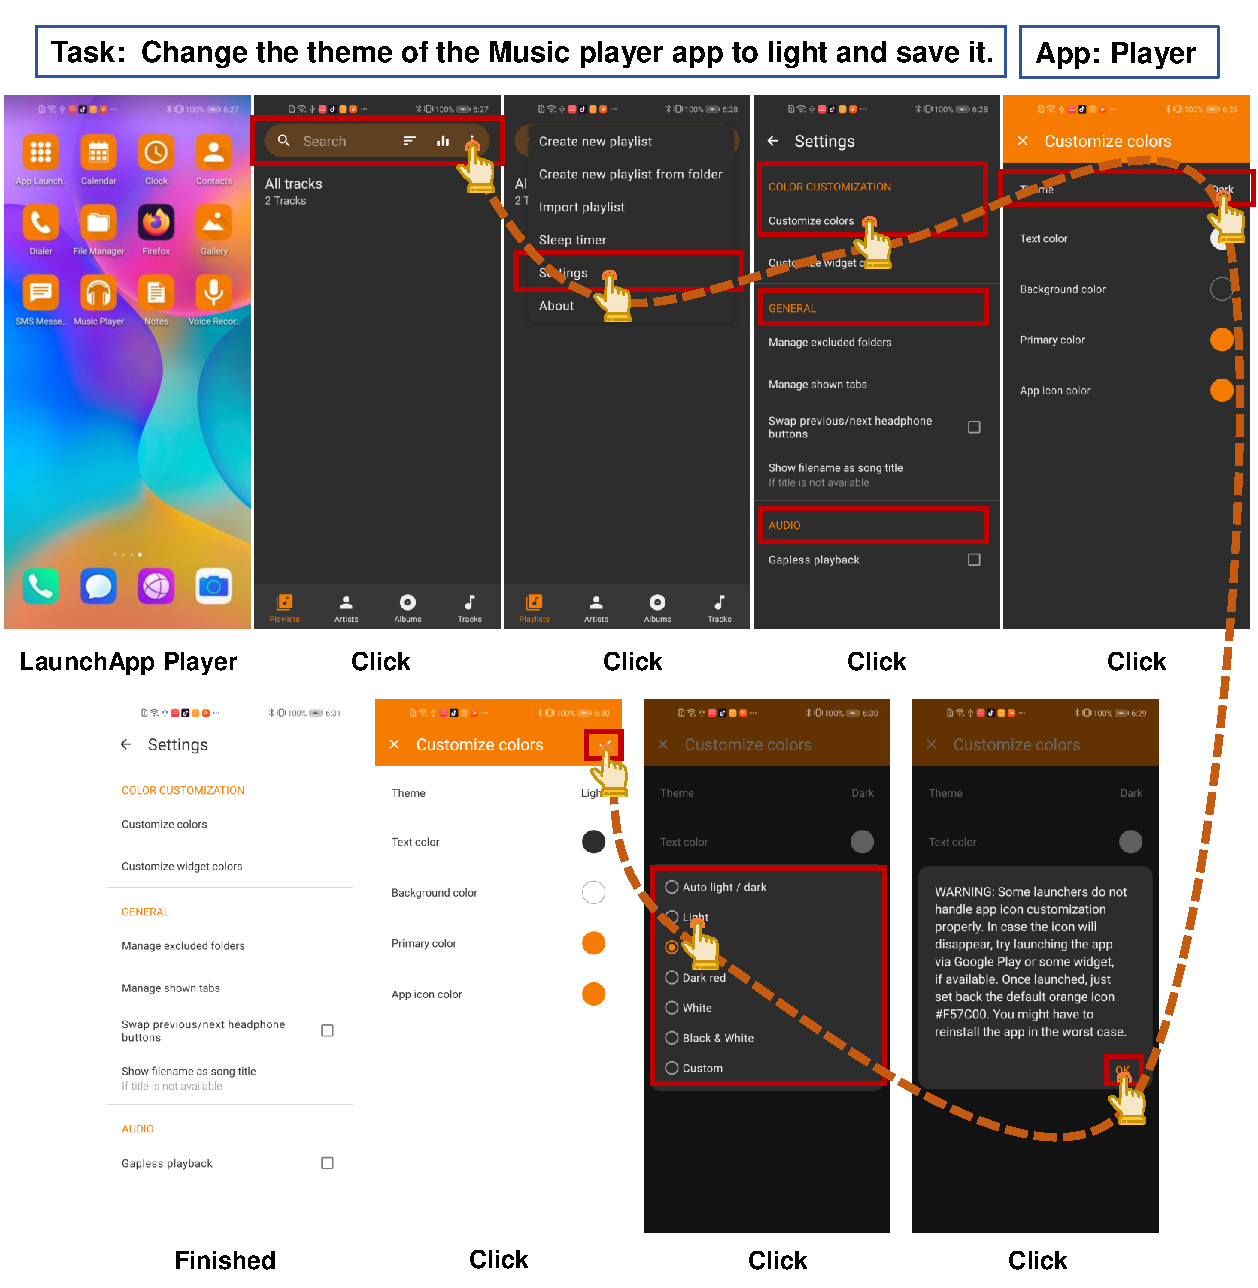
\includegraphics[width=0.8\textwidth]{pics/case3.pdf}
    \caption{A case of customizing the color theme in the Player app. The task is completed with reduced UI exposure; only UI content within the red boxes is transmitted to the cloud.}\label{fig:case3}
\end{figure}

\begin{figure}[htbp]
    \centering
    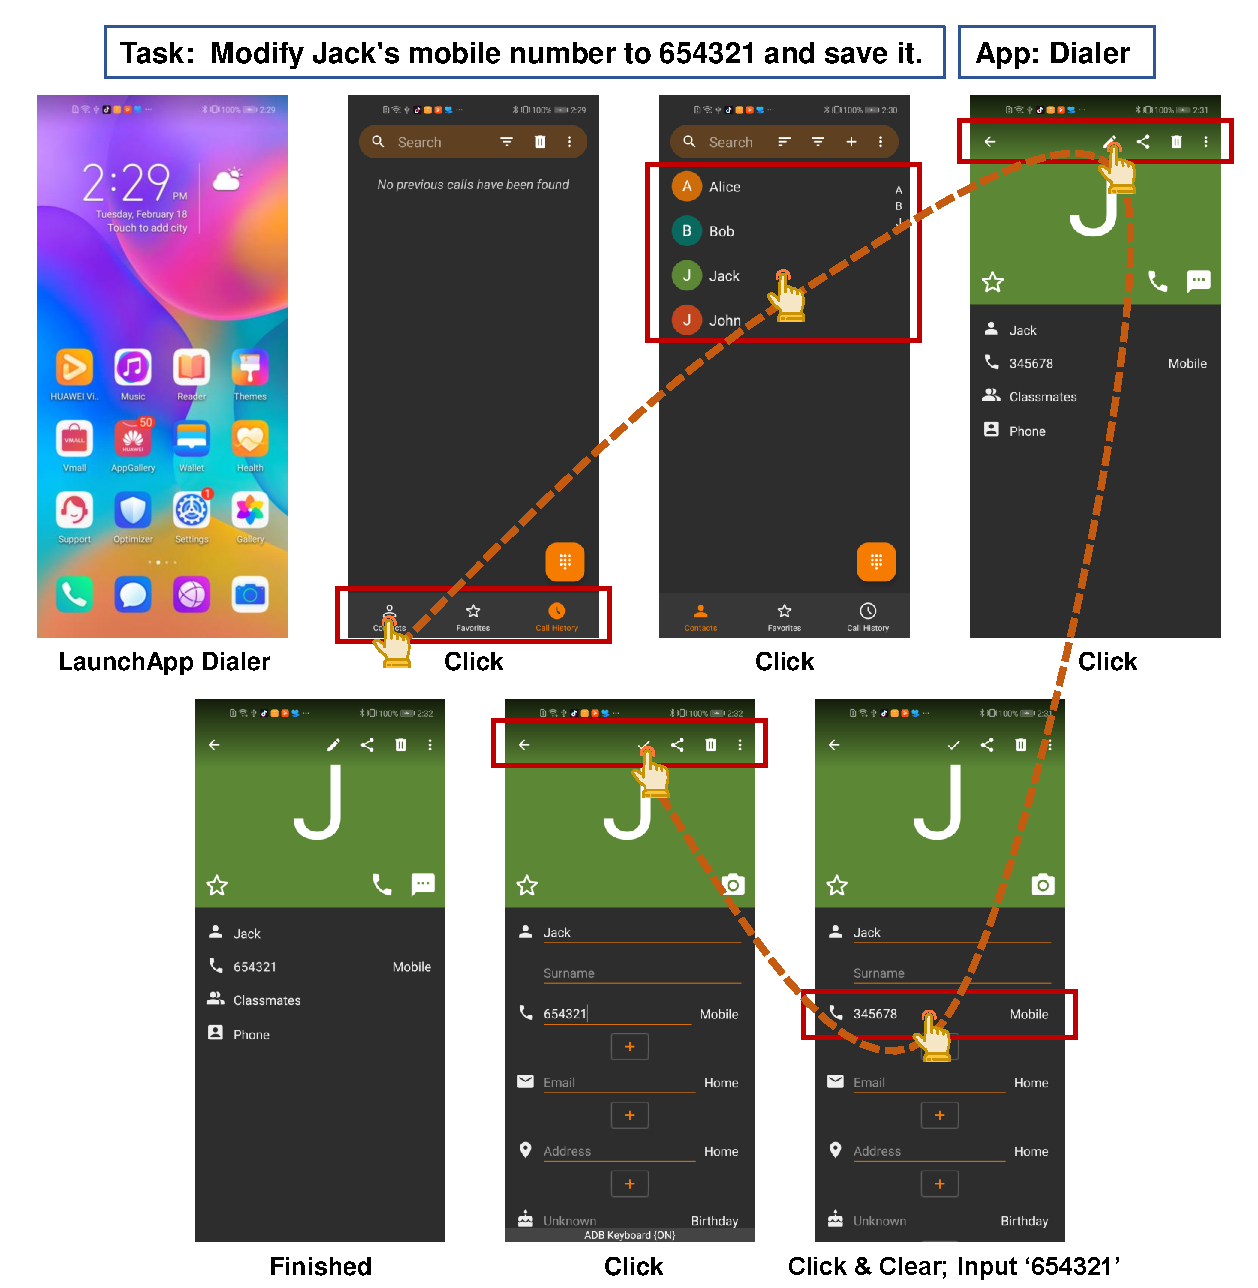
\includegraphics[width=0.74\textwidth]{pics/case1.pdf}
    \caption{A case of updating a contact's phone number in the Dialer app.}\label{fig:case1}
\end{figure}

\begin{figure}[!htbp]
    \centering
    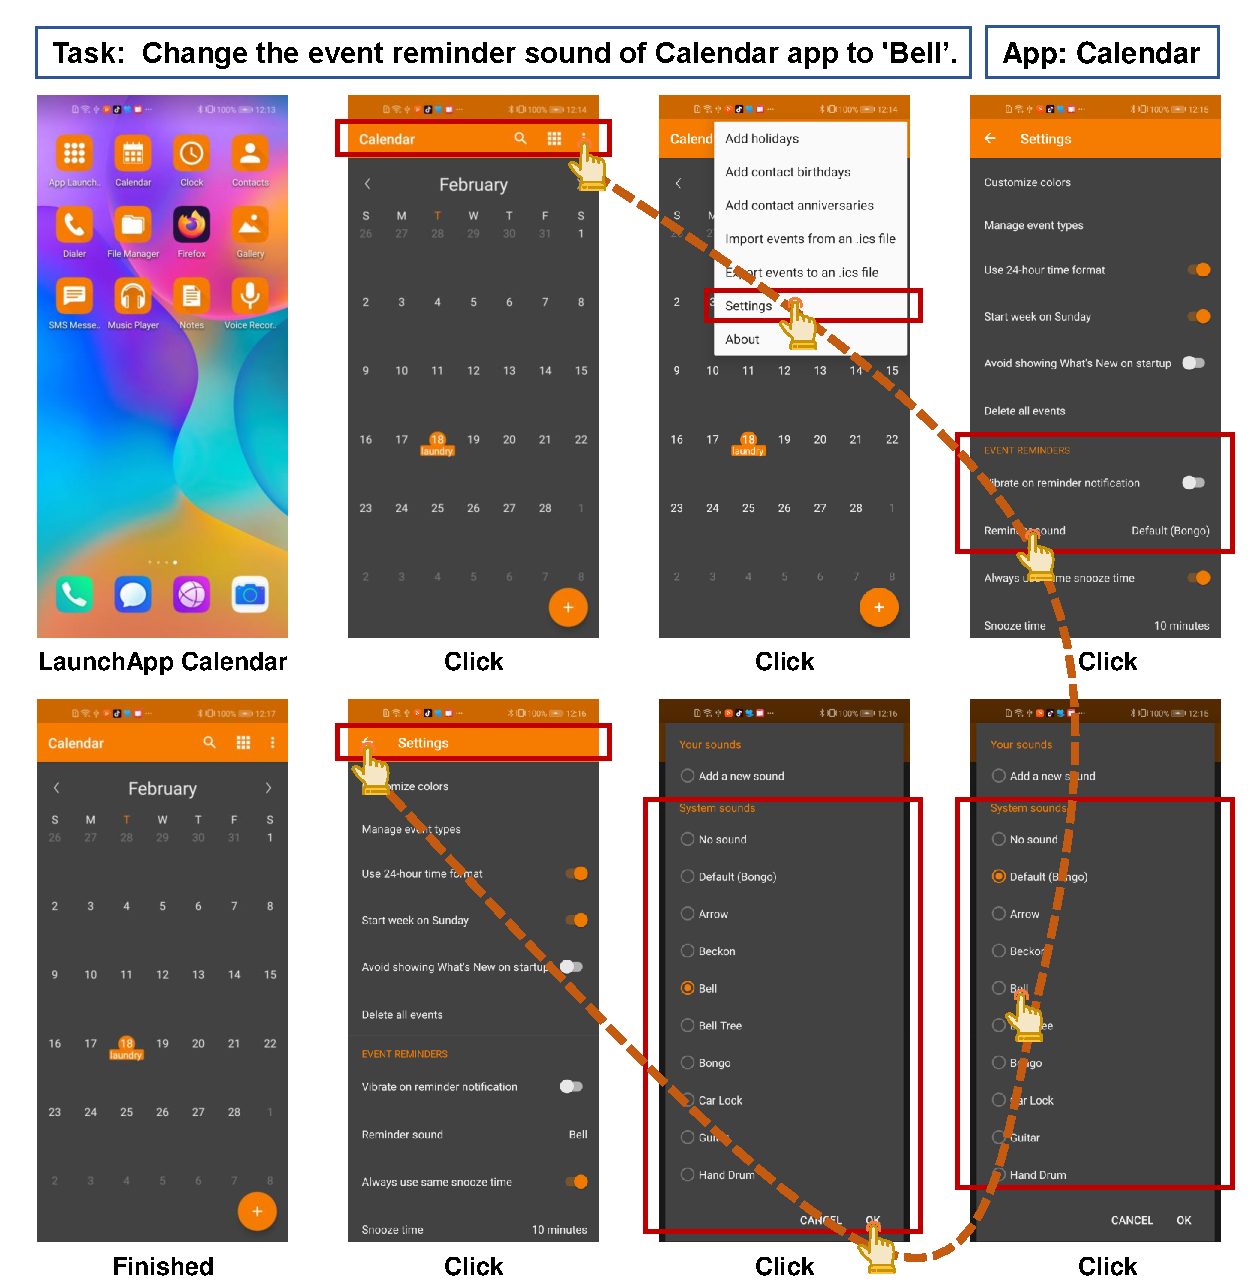
\includegraphics[width=0.74\textwidth]{pics/case2.pdf}
    \caption{A case of changing the reminder sound in the Calendar app.}\label{fig:case2}
\end{figure}

\begin{figure}[!htbp]
    \centering
    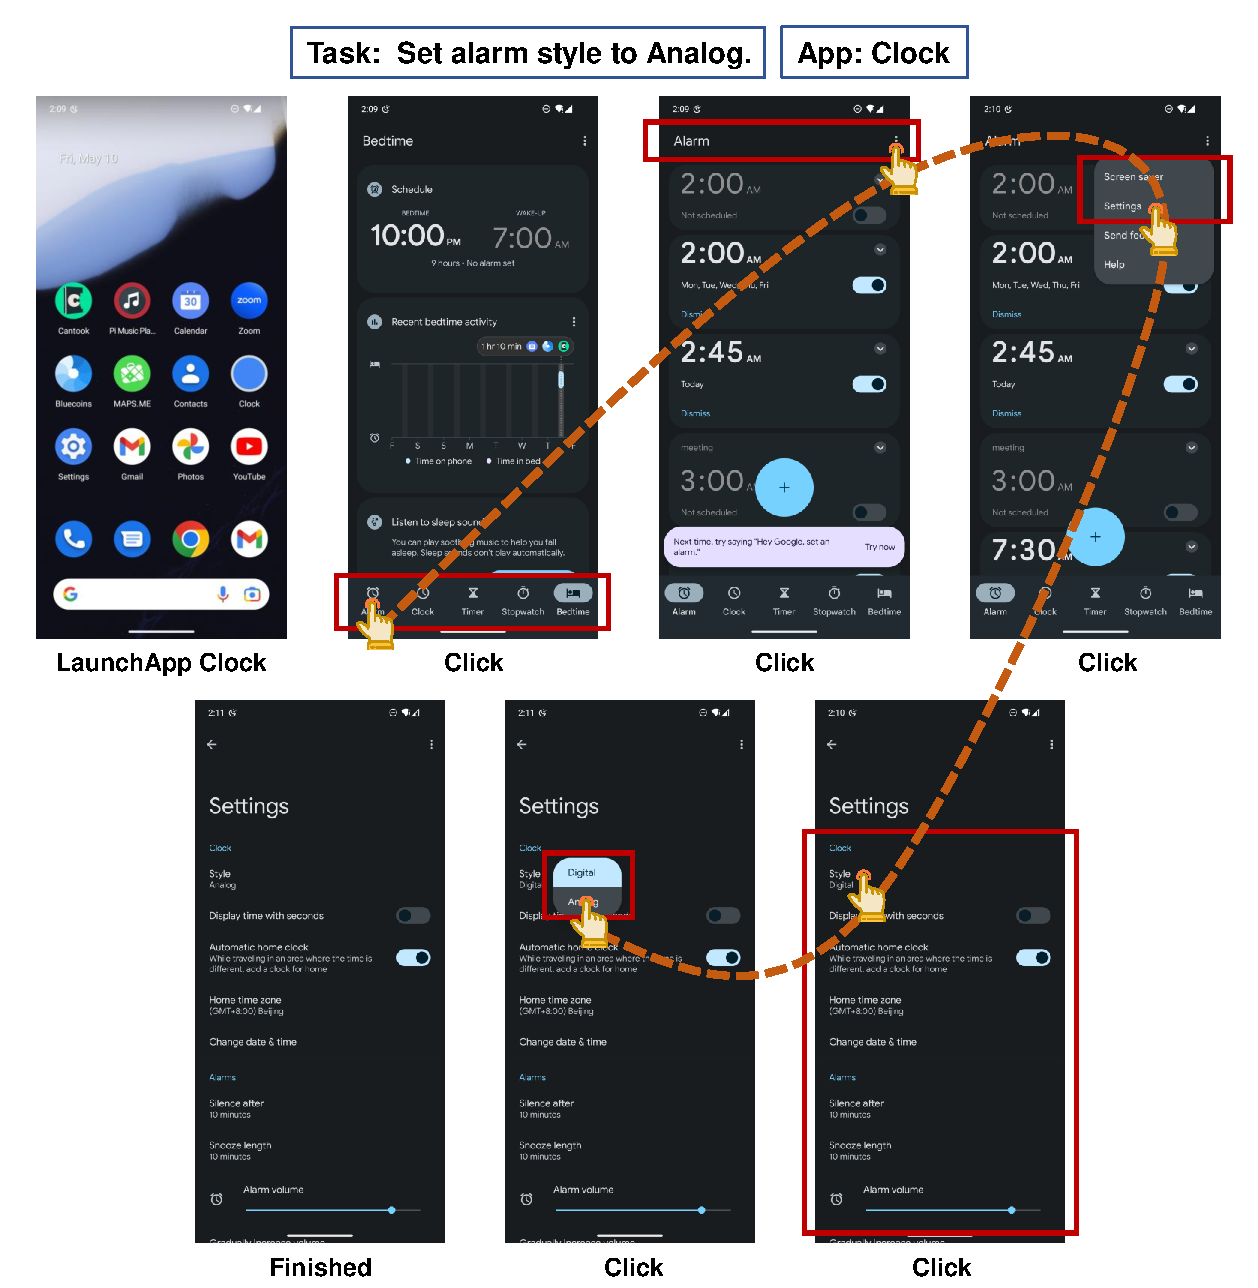
\includegraphics[width=0.74\textwidth]{pics/case4.pdf}
    \caption{A case of setting the alarm type in the Clock app.}\label{fig:case4}
\end{figure}

\begin{figure}[!htbp]
    \centering
    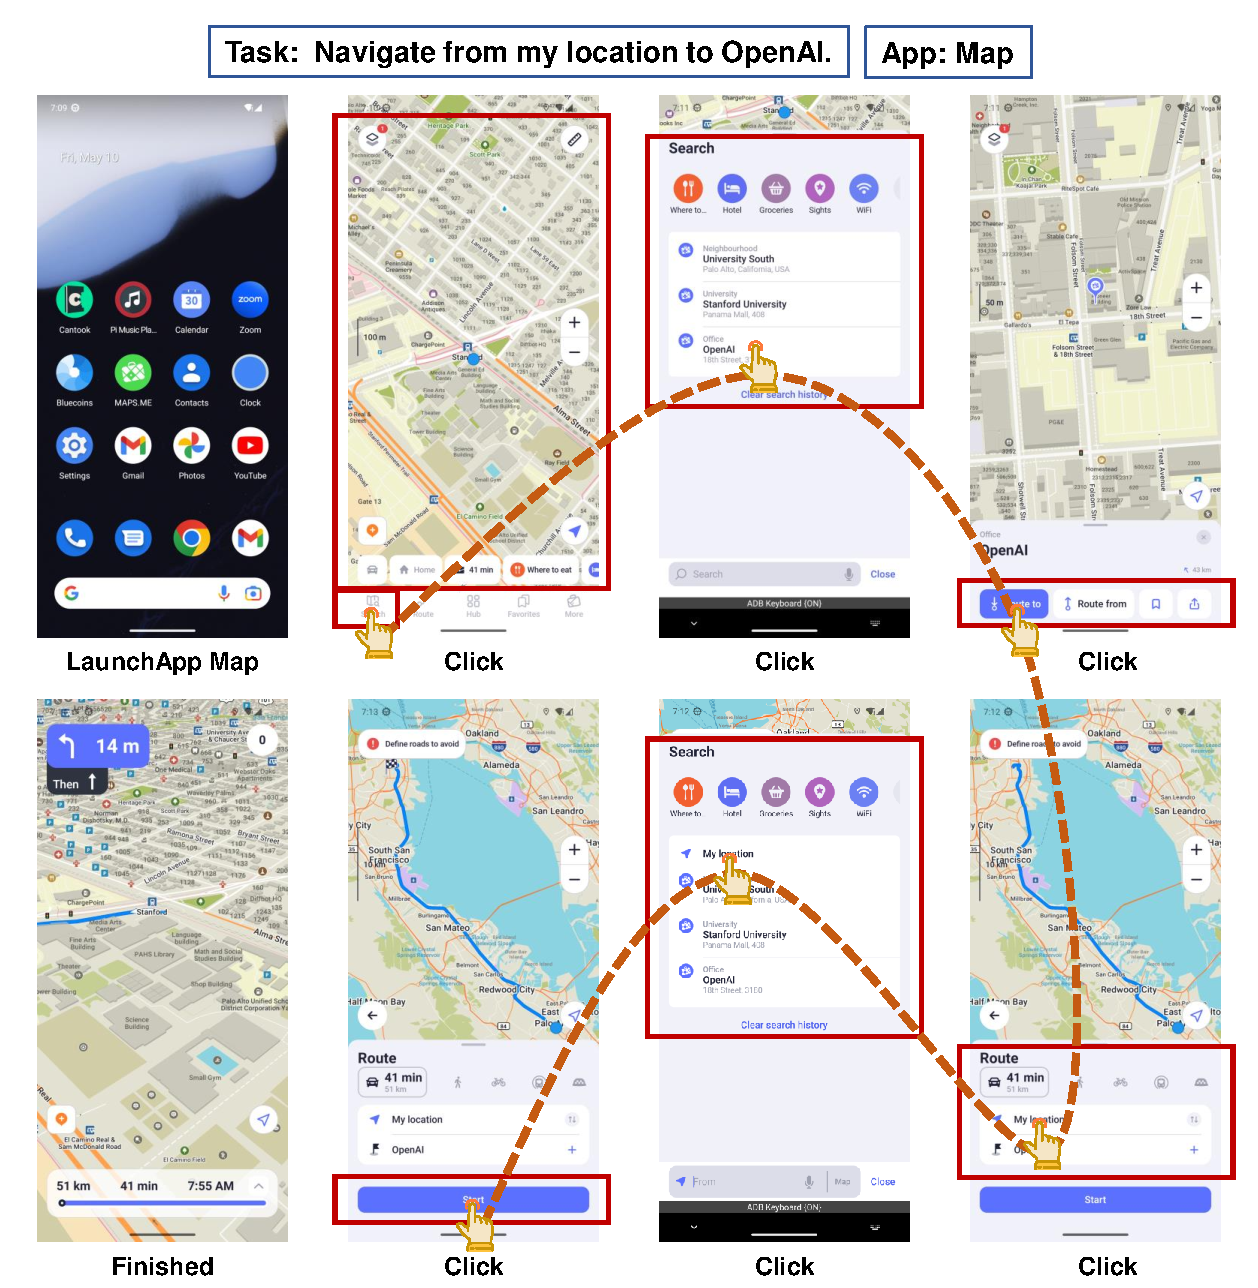
\includegraphics[width=0.74\textwidth]{pics/case5.pdf}
    \caption{A case of navigation in the Map app.}\label{fig:case5}
\end{figure}

\section{Case Study}
We illustrate five representative examples in Figures~\ref{fig:case3}--\ref{fig:case5} (three tasks from the DroidTask dataset \citep{wen2024autodroid} and two from the AndroidLab dataset \citep{xu2024androidlab}). The agent first triggers the main activity of an app to start. A hand icon indicates user-like interactions with UI elements on the screen executed by the mobile agent, and orange dashed lines represent the sequence of interactions, continuing until our framework determines task completion during co-planning. Our framework is XML-based, which extracts attributes of UI elements (e.g., \texttt{text}, \texttt{content-desc}, \texttt{bounding box}) from XML nodes, without relying on visual screenshots. However, for better illustration of UI exposure reduction, we visualize the subset of UI content uploaded to the cloud with red solid bounding boxes. UI elements outside these boxes are excluded from transmission to the cloud, representing the reduced exposure achieved by our method.

Overall, these tasks are successfully completed with little UI exposure. The reduction ratio in each round varies, depending on the UI layout and the number of UI blocks that the cloud LLM needs to make a confident decision on the current sub-task.